\chapter{Pensamento Computacional}\label{pensamento-computacional}

\section{Computadores e as transformações na prática científica}
% A evolução da computação nos últimos anos, aliado ao seu barateamento, tem tornado possível o desenvolvimento de novas estratégias para resolução de problemas. Fato que tem produzido impactos notáveis tanto na academia quanto nas empresas.

% barateamento de capacidades computacionais de armazenamento e processamento

% As últimas 2 ou 3 décadas dominado - e o mundo transformado - pelo advento de computação cada vez mais poderosa, menos dispendiosa e onipresente, além do surgimento da World Wide Web e tecnologias relacionadas.


A evolução da computação nas últimas décadas, aliada ao seu barateamento, tem produzido impactos notáveis tanto na academia quanto na industria. A disponibilidade de dispositivos mais baratos e com maior capacidade de processamento e armazenamento tem tornado a computação ubiqua. 

% **Enriquecimento das formas de exploração de fenômenos.**

Na academia, esse fenômeno tem favorecido o surgimento de novas estratégias para exploração de fenômenos. Até meados do século 20, todo progresso cientifico foi conduzido apenas por interações entre atividades experimentais e analíticas\footnote{
Em sentido mais amplo, quando mencionamos `atividade analítica' estamos nos referindo à utilização de aparato matemático para resolução teórica de problemas. Ao mesmo tempo, o termo análise também pode fazer referência ao emprego da análise matemática, ramo da matemática que lida com conceitos do cálculo diferencial, tais como diferenciação, integração, e séries infinitas.}. O surgimento da computação e o seu desenvolvimento desde então trouxe consigo novas formas de fazer ciência, tais como a simulação e a modelagem computacional, e mais recentemente, a mineração de dados e o aprendizado de máquina, úteis para a análise de grande volume de informação \cite{Djorgovski2005, wing2006}. %TODO (cite weintrop, and wing)


O uso de simulações numéricas, por exemplo, se justifica ao permitir que um grande número de fenômenos muito complexos sejam analiticamente tratáveis. Em muitos casos essa é única forma de exploração possível. Mesmo na mecânica newtoniana mais simples, é possível resolver  exatamente, apenas, o problema de dois corpos. Para $N\geq3$, soluções numéricas são necessárias. Da astronomia podemos retirar alguns exemplos, como a formação de estrelas e galáxias e explosão estrelares - de modo geral, qualquer evento envolvendo turbulência  \cite[]{Djorgovski2005}. %weintrop

O uso de métodos computacionais, tal como a simulação, tem expandido a abrangência de sistemas não lineares que tem sido explorados pelo modelos matemáticos e computacionais. Como lembra \citeonline{Weintrop2016}, campos da ciência estão experimentando um renascimento de abordagens experimentais em razão do acesso facilitado a mais poder computacional. 

O autor destaca que num passado recente, para muitos pesquisadores apenas o estudo de sistemas determinísticos era viável, tendo o termo `não-linear', praticamente, o sinônimo de `insolúvel'. Havia desse modo a propensão à investigação computacional apenas de sistemas lineares. Esse quadro era especialmente verdade para muitas pesquisas em biologia e química. 

Esse processo ganha especial relevância ao nos darmos conta da natureza caótica da ampla maioria dos fenômenos físicos. Sistemas lineares e determinísticos são portanto exceções, e não a regra \cite[]{Weintrop2016}.

Outros agentes de transformações da prática científica, embora mais recentes e em fase nascente, são as novas possibilidades trazidas pela abundância e pelo barateamento do armazenamento grandes volumes de dados. Vivemos uma era onde a disponibilidade de dados gerados por câmeras, sensores, execução de simulações e registro de interação humana crescem exponencialmente. 

Nesse cenário, como ressalta \citeonline[]{Djorgovski2005}, o foco de valores tem mudado da propriedade de dados ou de instrumentos para reuni-los para a propriedade de conhecimento e ideas que tornam possíveis a extração de significados desse volume de informação. 

A abundância traz consigo muitos desafios. A taxa com que cientistas e engenheiros têm coletado e produzido dados vem exigindo avanços nas estratégias de análise. O acúmulo chegou a um nível de complexidade que, certo modo, tem sido impossível fazer qualquer tipo de investigação superficial utilizando técnicas convencionais, baseadas na percepção humana. Lidar com esse conjunto desestruturado e rico de dados, extraindo dele significado, tem sido uma das batalhas da atual revolução científica e industrial \cite[]{Djorgovski2005}. Nesse contexto o emprego de técnicas de aprendizado de máquina é essencial.

Em linhas gerais, o aprendizado de máquina (do inglês: \textit{machine learning}) baseia-se no uso algoritmos que instruem computadores como avaliar dados e deles extrair padrões e correlações, permitindo-os, de forma extraordinária, a fazer predições. E esse processo tem um componente recursivo: quanto mais análises são feitas, mais experiência e competência são adquiridas. Ou seja, mais `inteligentes' essas máquinas se tornam.

\citeonline[]{Escobar} propõe uma visão simplificada das interações humanas que facilita o entendimento desses algoritmos. Como descreve, ao conhecemos alguém pela primeira vez, baseando-nos em modelos pessoais, somos capazes de dizer nos primeiros minutos se essa pessoa nos transmite boa ou má impressão. Para cada nova pessoa que encontramos, avaliamos algumas de suas características e as registramos. Esse processo nos permite refinar e recompor modelos sociais que irão influenciar outras percepções em interações futuras. 

É exatamente nesse princípio recursivo que se fundamenta o aprendizado de máquina: categorizar dados de acordo com suas características com o fim de compor e refinar modelos.

Esse processo tem se provado extremamente eficiente na predição da configuração de sistemas estocásticos. Tomemos por exemplo a necessidade de prever o tempo, onde há dominância de comportamentos turbulentos. Em um estudo recente \apud[]{PhysRevLett.120.024102}{Vutha}, mostrou-se a eficiência do uso de algoritmos de inteligência artificial para previsões ao longo de um período muito maior do que se imaginou possível. Um ponto digno de nota: o algoritmo utilizado não continha nenhuma informação sobre as equações subjacentes. 

Há atualmente questionamentos sobre até que ponto o uso intensivo de `robôs oráculos' levará à perda do interesse dos pesquisadores em descrever fenômenos em termos de equações e princípios unificadores. Esse debate é sintetizado pela confronto das noções de ``predição'' e ``entendimento''.

\citeonline[]{Vutha} expõe os elementos desse debate com um exemplo histórico. Como destaca, durante mais de um milênio, o movimento dos planetas eram descritos a partir de um modelo elaborado por Ptolomeu, cujos métodos lançavam mão de cálculos misteriosos envolvendo sobreposição de círculos. Apesar de ignorar a teoria da gravidade e de ter a Terra no centro do Universo, essa representação foi extremamente eficiente na sua capacidade preditiva. Ao mesmo tempo, pode-se dizer que ela era incompleta na medida em que não oferecia nenhum entendimento capaz de explicar o seu funcionamento.

\begin{figure}[htb]
	\caption{\label{Ptolomeu} Modelo geocêntrico de Ptolomeu}
	\begin{center}
	    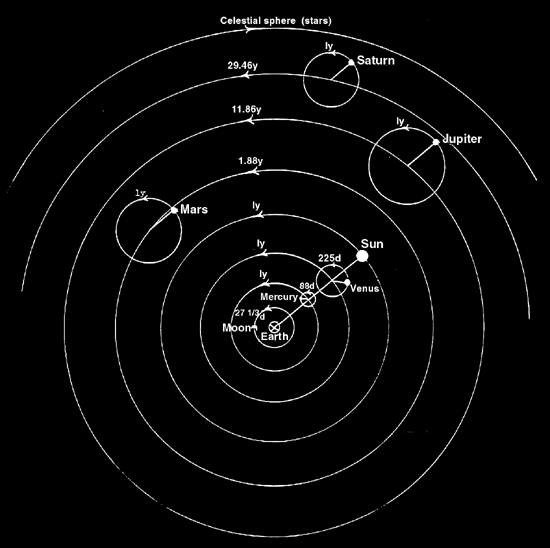
\includegraphics[scale=0.5]{imagens/ptolemy}
	\end{center}
	\legend{Fonte: \citeonline[]{Hatch}}
\end{figure}

A descrição do movimento dos corpos celestes só foi finalmente compreendida a partir da equações diferenciais descobertas por Isaac Newton. Com elas tem sido possível, desde então, prever a trajetória de todo e qualquer planeta do sistema solar.

A qualidade da proposta de Newton estava na possibilidade de oferecer não apenas a descrição de trajetórias, mas por permitir também que entendamos o porquê que elas são de uma e não de outra forma. Ao nos trazer equações, ele nos facultou a compreensão do fenômeno do movimento a partir da ótica de princípios unificadores. E é exatamente nesse ponto que reside o poder da descrição matemática. Como analisa \citeonline{Vutha}, se formos capazes de extrair de um fenômeno complicado dois ou três princípios, podemos dizer então que o compreendemos.
 

Porém, dada a dominância de fenômenos complexos na natureza, tem sido extremamente difícil extrair de muitos deles princípios simples. Descrevê-los, portanto, a partir da obtenção de equações universalmente válidas pode ser uma forma um tanto ineficiente de gerar predições relevantes \cite{Vutha}. O emprego de técnicas de \textit{machine learning}, nesse sentido, tem sido essencial.

A inteligência artificial tem ocupados outros espaços além da pesquisa científica. Desde robôs que leem a web para tomar decisão de investimentos \cite[]{Bloomberg} e carros que se auto dirigem, até contextos relativamente mais simples como tradutores automáticos e mecanismo buscas. Já no mundo do trabalho, um sem-número de projeções apontam para a substituição progressiva de quantidade considerável de atividades laborais por robôs.


\begin{figure}[htb]
	\begin{center}
	    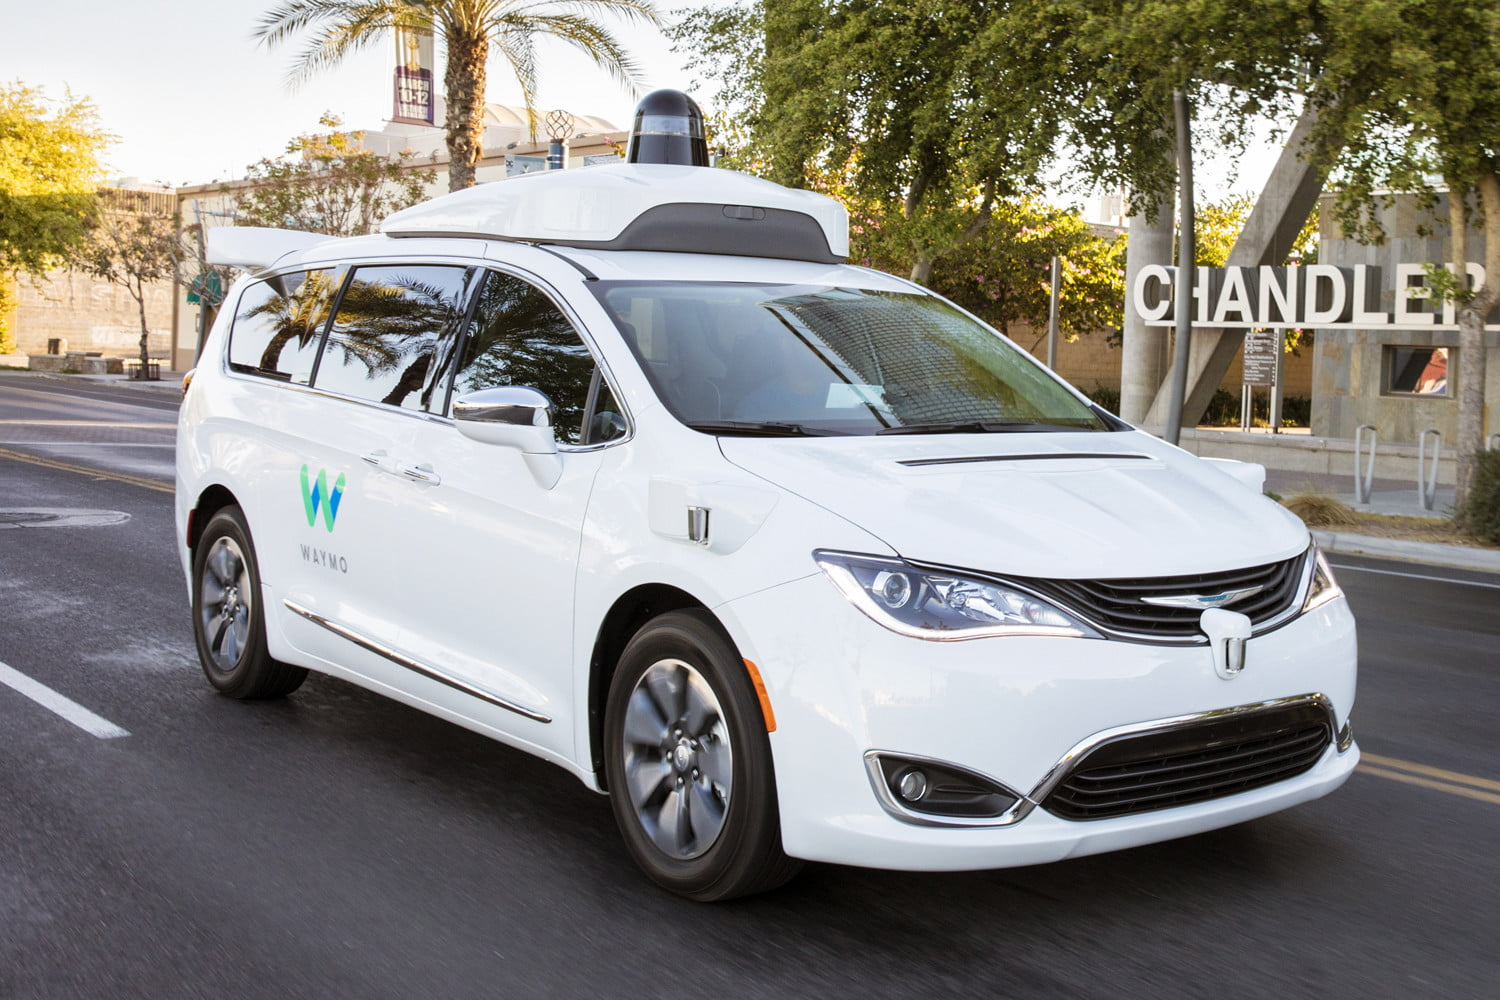
\includegraphics[scale=0.25]{imagens/waymo}
	\end{center}
	\caption{\label{Waymo} Carro autônomo da Waymo, subsidiária de veículos da Alphabet (matriz do Google)}
\end{figure}

A produção estratosférica de dados e a invasão da inteligência artificial nos meios científicos e na indústria é sintomático da interação dinâmica entre a ciência, a tecnologia, e a sociedade em ciclos que se retroalimentam.

Novas descobertas levam a novas perguntas que exigem mais coleta de dados. Quando analisadas, essas informações são utilizadas para refinar e ajustar modelos, levando a novas perguntas e mais produção de dados. Esse processo tende a culminar na criação de novas tecnologias. Tecnologias, por seu turno, inspiram usos sociais criativos que quase sempre criam demandas por mais descobertas científicas e mais tecnologia. Sob esse aspecto, podemos dizer que esses três atores desempenham o papel de forças motrizes da computação \cite[]{wing2008}. 

\begin{figure}[htb]
	\caption{Forças motrizes da computação}
	\begin{center}
	    
\includegraphics[scale=0.28]{imagens/forcas_motriz.png}
	\end{center}
	\legend{Adaptado de \citeonline[]{wing2008}}
\end{figure}

O barateamento dos custos de produção científica é outro aspecto relevante dessas transformações. À medida que a internet e dados, consequentemente, se tornam mais acessíveis, qualquer pessoa com boas ideias e bons hábitos de trabalho, de qualquer lugar, pode fazer ciência de primeira linha, comunicar seus resultados e aprender com a comunidade científica. Essa possibilidade é especialmente benéfica para países e instituições que não dispõem de instalações de pesquisa sofisticadas \cite[]{Djorgovski2005}. 

Sobre o papel da ciência da computação no desenvolvimento científico, \citeonline[]{Djorgovski2005} faz um consideração provocativa: 

\begin{citacao}
	$[...]$ a ciência da computação aplicada está desempenhando o papel que a matemática fez do século XVII ao século XX: fornecer uma estrutura ordenada e formal e um aparato exploratório para outras ciências. Além de seu aparentemente feliz caso com a teoria das cordas, é difícil dizer o que a matemática está fazendo para outras ciências hoje. A maioria dos cientistas de matemática que utilizamos hoje foi desenvolvida há mais de um século. \cite[p.~131. Tradução nossa]{Djorgovski2005}
\end{citacao}

E é do do seio dessa reflexão que nasce a noção de um ``pensamento computacional''. Tema que desdobraremos a seguir.

\vspace{1cm}

\section{A consolidação da ciência da computação na investigação científica: o pensamento computacional}

A noção de pensamento computacional tem ganhado força desde 2006, ano em que a professora Jeannette Wing, então professora da Universidade Carnegie Mellon, publica um artigo seminal no qual propõe um conjunto de atitudes, ou abordagens, para a resolução de problemas fundamentadas na forma como cientistas da computação e programadores tratam problemas computacionais. 

A definição clássica que muitos autores dão para o conceito é extraído do próprio trabalho da autora que estabelece que pensamento computacional consiste ``numa abordagem para a solução de problemas, desenho de sistemas e entendimento do comportamento humano que se vale de conceitos fundamentais para ciência da computação'' \cite[Tradução nossa]{wing2006}, ou ainda, na capacidade de formular problemas e expressar suas soluções de forma suficientemente clara de tal modo que um computador possa executá-las.

O desenvolvimento do tema requer algumas discussões preliminares. Comecemos com uma apresentação sobre o papel dos algoritmos.

Em termos simplificados, um algoritmo nada mais é do que uma solução para um problema que satisfaz as seguintes condições \cite{Piwek2016}:

\begin{itemize}
	\item deve apresentar uma lista sequenciada de passos que levam à solução do problema 
	\item deve ser um processo finito
	\item deve resolver qualquer instância do problema em questão
\end{itemize}

\begin{figure}[htb]
	\caption{Algoritmo de soma de três números inteiros}
	\begin{center}
	    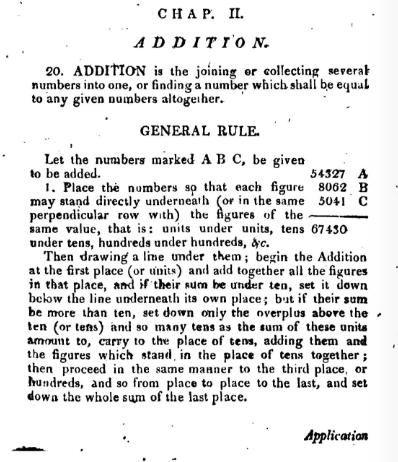
\includegraphics[scale=1]{imagens/algorithm.png}
	\end{center}
	\legend{Fonte: \citeonline{Gough}}
	\label{fig:algoritmo}
\end{figure}

Na figura \ref{fig:algoritmo} lê-se um conjunto de instruções para somar três números inteiros, extraídos do livro \textit{Practical Arithmetick in Four Books} do autor John Gough, publicado pela primeira vez em 1767. Sob o título `General rules', lemos

\begin{citacao}
	Coloque os números de modo que cada algarismo possa ficar diretamente abaixo (ou na mesma linha perpendicular) dos algorismos de mesmo valor, ou seja: unidades em unidades, dezenas em dezenas, centenas em centenas.$[...]$Em seguida, desenhando uma linha abaixo deles; comece a adição no primeiro lugar (ou unidades) e some todas os algorismos naquele lugar, e se a soma delas for menor que dez, coloque-a abaixo da linha abaixo de seu próprio lugar;mas se a soma for superior a dez, estabeleça apenas o excedente acima das dez (ou dezenas) e algumas dezenas, à medida que a soma dessas unidades se eleva, carregue para o local das dezenas, adicionando-as e os algorismos que estão no lugar de dezenas juntos; em seguida, proceda da mesma maneira até o terceiro lugar, ou centenas, e de um lugar para outro até o último, e estabeleça a soma total do último lugar.  
\end{citacao}

Perceba como essas instruções satisfazem as condições elencadas anteriormente: nela vemos um problema (cálculo da soma de três número inteiros) sendo resolvido de forma encadeada ao longo de um processo finito. Nota-se também que os passos acima facultariam a soma de quaisquer outros três números inteiros, atendendo a exigência de ``resolver qualquer instância do problema''. 

A tarefa de definir as instâncias de um problema equivale a delimitar qual é o seu escopo, ou seja, o alcance que uma possível solução deve atingir. Ao redigirmos um algoritmo para a divisão entre $a$ e $b$, por exemplo, deveríamos impor que ambos devem assumir quaisquer valores reais contanto que $b$ seja diferente de zero. Assim, ditamos os limites do problema, em outras palavras, as sua instâncias. Do ponto de vista da ciência da computação, ao procedermos dessa forma, distinguindo claramente os contornos de um problema, estamos definindo um ``problema computacional''.

A definição clara das instâncias do problema (criação de um problema computacional) e dos passos exatos para sua solução\footnote{Ao tratarmos computacionalmente um problema devemos ser capazes também de distinguir quando e porque, eventualmente, ele não tem solução.} (elaboração de um algoritmo) nos permitirá automatizar a sua execução por um computador. E é exatamente nessas duas habilidades, conforme definição dada anteriormente, que se apoiam o pensamento computacional.

A noção de abstração é outro componente que necessita ser compreendido ao tratarmos do assunto. Nas palavras de \citeonline{wing2006},

\begin{citacao}
A abstração é usada na definição de padrões, generalização de instâncias e parametrização. É usado para deixar um objeto representar muitos. Ele é usado para capturar propriedades essenciais comuns a um conjunto de objetos enquanto oculta distinções irrelevantes entre eles \cite[p.~1. Tradução nossa]{wing2006}
\end{citacao}

Abstrair, como enfatiza o trecho acima, equivale simplesmente a conduzir um processo de generalização, onde incorporamos parte dos detalhes da realidade em um modelo, ao mesmo tempo que descartamos outros. Estabelece-se assim uma relação entre dois níveis: a realidade e sua representação.

\begin{figure}[htb]
	\caption{Relação entre a realidade e o seu modelo}
	\begin{center}
	    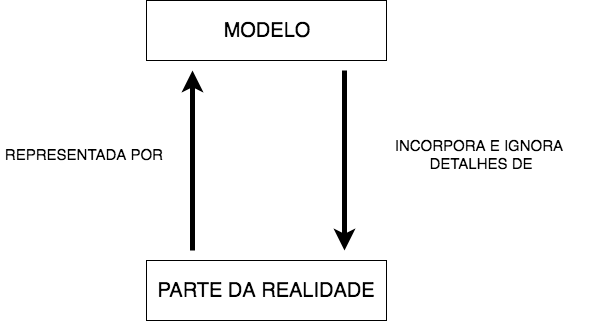
\includegraphics[scale=0.65]{imagens/modelo_e_realidade.png}
	\end{center}
	\legend{Adaptado de \citeonline[]{Piwek2016}}
\end{figure}

A figura \ref{fig:pipe} ilustra essa discussão. Nela vemos a obra ``A Traição das Imagens '' por René Magritte (1898-1967), onde lê-se \textit{``Ceci n'est pas une pipe''} (``Isto não é um cachimbo''). Temos aí provocação que evidencia que um modelo nada mais é do que uma representação, e não a realidade em si.

\begin{figure}[htb]
	\caption{``A Traição das Imagens'' por René Magritte, 1929}
	\begin{center}
	    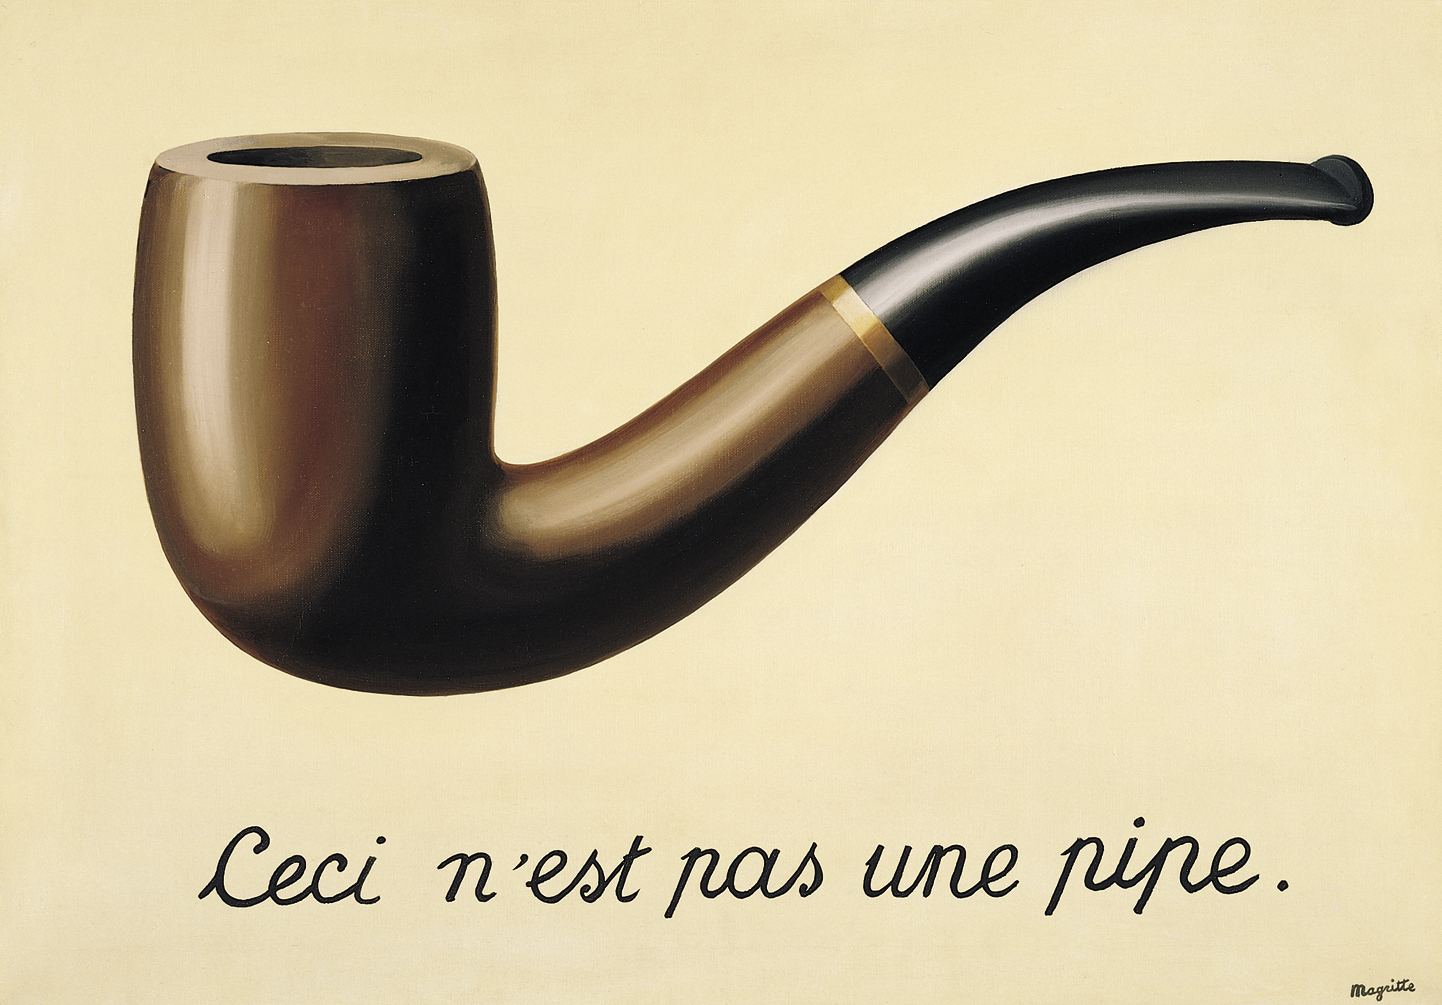
\includegraphics[scale=0.75]{imagens/pipe}
	\end{center}
	\label{fig:pipe}
\end{figure}

O grau de detalhamento do modelo depende das circunstâncias do problema, bem como das necessidades de quem modela. Por exemplo, ao analisarmos a trajetória de lançamento de um foguete, podemos descartar suas dimensões e eliminar possíveis efeitos aerodinâmicos. Essa abordagem é extremamente conveniente para o ensino de primeiras noções de física básica, mas demasiadamente simplória no contexto da condução de um programa aerospacial.

Na figura \ref{fig:cows} temos a ilustração dessa ideia: a mesma ``realidade'' vaca representada por quatro modelos com diferentes graus de detalhes incorporados.

\begin{figure}[htb]
	\caption{Quatro representações de uma vaca por Theo van Doesburg, 1917--1918}
	\begin{center}
	    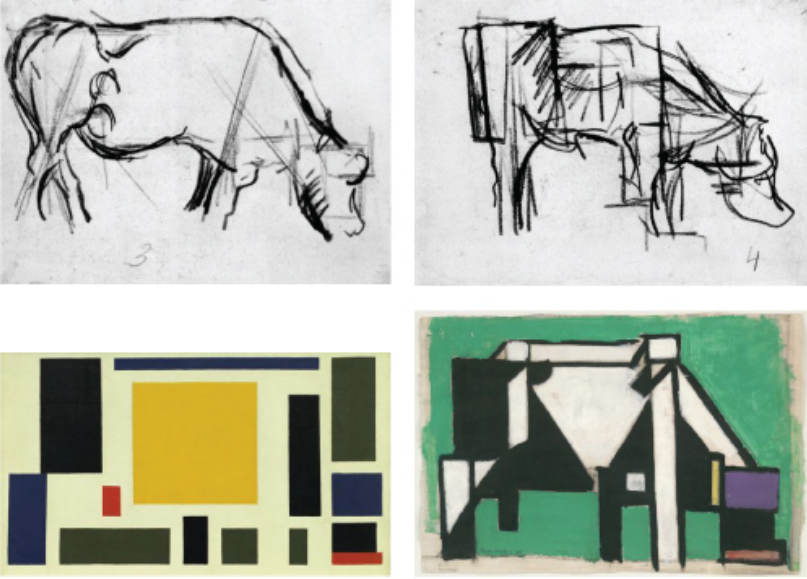
\includegraphics[scale=0.26]{imagens/vacas.png}
	\end{center}
	\legend{Fonte: \citeonline[]{Piwek2016}}
	\label{fig:cows}
\end{figure}

É interessante notar a proximidade do significado para abstração discutido até aqui com aquele proposto pelo filósofo John Locke, segundo o qual formação de uma abstração corresponde a uma transformação durante a qual ``ideias tomadas de seres particulares se tornam representantes gerais de todos do mesmo tipo'' \apud[p.~354. Tradução nossa]{Locke}{Sengupta2013}.

\citeonline[]{Piwek2016} distingue dois tipos de abstrações: a ``abstração como modelo'', onde detalhes da realidade observada são desconsideradas em favor de outras -- o mesmo trabalhado até aqui -- e a ``abstração como encapsulamento'', processo no qual organizamos nosso modelo em módulos ou cápsulas que permitem a composição de sistemas mais complexos. 



Para diferenciarmos esses dois tipos tomemos como ponto de partida o planetário mecânico ilustrado na figura \ref{fig:planetario}. Nele vemos uma simulação\footnote{Usamos o termo \textbf{simulação} para nos referir a modelos que incorporam uma representação da evolução temporal de um processo ou sistema.} do sistema solar, um modelo, que como tal ignora certas aspectos da realidade. Neste caso em específico temos a desconsideração típica de representações astronômicas onde as proporções entre as dimensões dos planetas e a distância relativas entre eles é extremamente grande. A construção de modelos, ignorando e incorporando detalhes, é o que \citeonline{Piwek2016} chama de ``abstração como modelo''. 

\begin{figure}[htb]
	\caption{Planetário mecânico}\label{fig:planetario}
	\begin{center}
		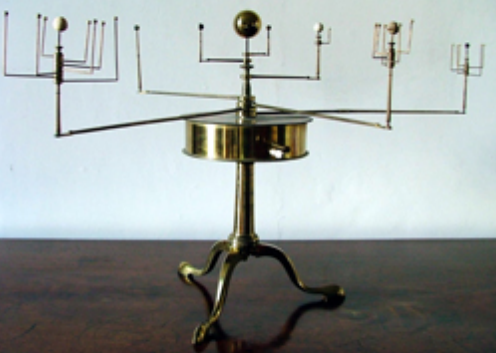
\includegraphics[width=0.50\textwidth]{imagens/planetario}
	\end{center}
	\legend{Fonte: \citeonline{Piwek2016}}
\end{figure}

O mesmo dispositivo incorpora a noção do que o autor chama de ``abstração como encapsulamento''. Na figura \ref{fig:engine} vemos um sistema de rodas dentadas típico do que podemos encontrar no interior de um planetário mecânico. São elas que permitem o movimento das esferas que representam os planetas. A superfície metálica que vemos na figura \ref{fig:planetario} cumprem o papel de interface do modelo ao escondê-las, deixando externamente visível apenas o que é relevante: o movimento de translação e rotação. 

\begin{figure}[!htb]
	\caption{Engrenagem de um planetário mecânico}\label{fig:engine}
	\begin{center}
		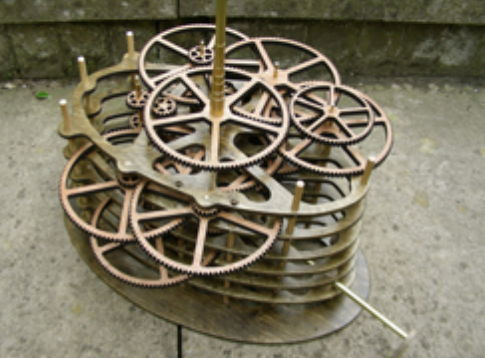
\includegraphics[width=0.50\textwidth]{imagens/engine}
	\end{center}
	\legend{Fonte: \citeonline{Piwek2016}}
\end{figure}

Distingue-se assim a formação de duas camadas durante o processo de encapsulamento: a interface com a qual se pode interagir com o modelo (o invólucro metálico do planetário) e a sua implementação propriamente dita (sistema de engrenagens encerradas pela interface). A figura \ref{fig:encapsulamento} ilustra a relação entre elas.

\begin{figure}[!htb]
	\caption{Interface e implementação - dois aspectos de um modelo}\label{fig:encapsulamento}
	\begin{center}
		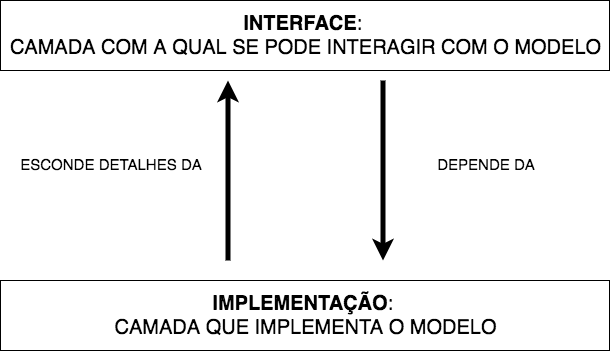
\includegraphics[scale=0.55]{imagens/encapsulamento}
	\end{center}
	\legend{Fonte: \citeonline{Piwek2016}}
\end{figure}







% $$divisão(2,3)$$












% Além de permitir a construções de modelos (abstração como modelos), a construção de abstrações agrupam outro conceito: `abstração'





% O trecho acima enfatiza a criação de uma abstração como um processo de generalização. Abstrações, desse ponto de vista, são representações generalizadas aplicáveis a diversos contextos ou situações. 

% significado filosífico. TODO: incluir

% É interessante notar a proximidade da conceptualização de Wing com a do inglês John Locke. Basicamente, o filósofo distinguia dois tipos de ideas: particulares e gerais. As primeiras, limitadas a contextos específicos no tempo e no espaço, enquanto as últimas, livres de tais restrições, poderiam ser aplicadas a configurações diversificadas. Nesse processo, a formação de uma abstração corresponde a uma transformação durante a qual ``ideias tomadas de seres particulares se tornam representantes gerais de todos do mesmo tipo'' \apud[p.~354. Tradução nossa]{Locke}{Sengupta2013}.

% No contexto da computação científica, o uso de abstrações se dá a partir da construção e do uso de modelos matemáticos. Estabelece-se aí a noção de abstração como modelagem. %mas 

% A necessidade de criação de um modelo nasce normalmente da intenção de se elaborar uma descrição de um sistema ou processo, como no caso das ciências físicas onde se buscam representações para fenômenos da realidade. 

%Essencialmente, ao construirmos um modelo buscamos 

%A tarefa de se construir 

%Ao decidirmos estudar um fenômenos procedemos ao levantamento do que é considerado relavante, descartando aspectos que menos essencias. 

%A criação de um modelo involve o destaque de aspecto relevantes ao mesmo tempo em que se realiza o descarte do que se considera menos essencial.








%Ao construirmos um modelo

%TODO - inserir ``four imag es of cow of theo van Doesburg''








